\subsection{Turbulent Transport}

\subsubsection{What are relevant physical time scales in turbulent flow? How do they relate to chemical time scales?}

{\color{gray}\footnotesize [Claude context: check Lecture 10 (Turbulence-Chemistry Interaction \& Modelling) and Lecture 8 (how turbulence affects combustion regimes); Warnatz Ch.13 (Turbulent Reacting Flows); JMBC course chapter 8 (Roekaerts)]}

\paragraph{Answer}
Lecture 8: time scales

Important timescales are the chemical $t_c$, the Kolmogorov $t_k$, and the large (or integral) $t_t$.

For turbulent flow, the large timescales relate to the chemical timescale through the turbulent Reynolds number, Re$_t$.

\begin{figure}[H]
    \centering
    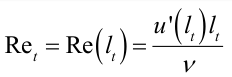
\includegraphics[width=0.75\linewidth]{exam-questions/03-turbulent-transport/Re.png}
    \caption{Definition of the turbulent Reynolds number $\mathrm{Re}_t$, relating the integral length scale $l_t$ and velocity fluctuation $u'(l_t)$ to the kinematic viscosity $\nu$.}
    \label{fig:re-number}
\end{figure}

The large and chemical timescales are related through the Damk\"ohler number.

\begin{figure}[H]
    \centering
    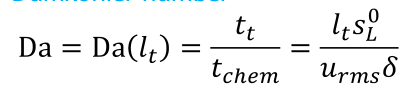
\includegraphics[width=0.75\linewidth]{exam-questions/03-turbulent-transport/Da.png}
    \caption{Definition of the Damk\"ohler number $\mathrm{Da}$ as the ratio of the integral (large-scale) timescale $t_t$ to the chemical timescale $t_{chem}$.}
    \label{fig:damkohler-number}
\end{figure}

The turbulent (Kolmogorov) and chemical timescales are related through the Karlovitz number.

\begin{figure}[H]
    \centering
    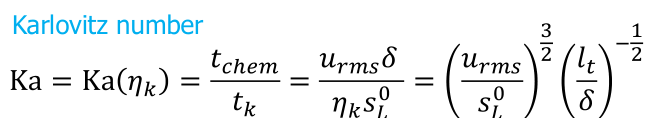
\includegraphics[width=0.75\linewidth]{exam-questions/03-turbulent-transport/karl.png}
    \caption{Definition of the Karlovitz number $\mathrm{Ka}$ as the ratio of the chemical timescale $t_{chem}$ to the Kolmogorov timescale $t_k$.}
    \label{fig:karlovitz-number}
\end{figure}

This sets up the different flame regimes, as seen in the Peters diagram.

The y-axis is the ratio of the turbulent velocity fluctuation to the unstretched flame speed (consumption speed), $u_{rms}/s_L^0$.

The x-axis is the ratio of the integral length scale to the unstretched flame thickness, $l_t/\delta$.


\begin{figure}[H]
    \centering
    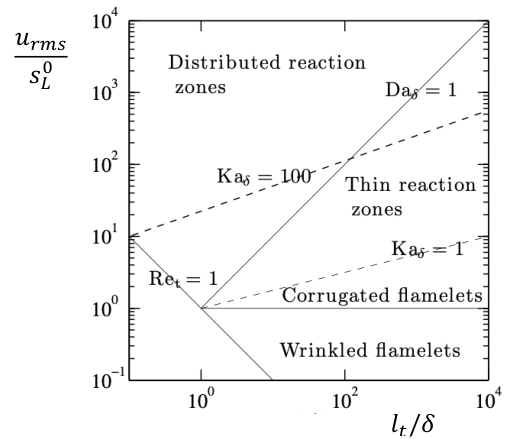
\includegraphics[width=0.75\linewidth]{exam-questions/03-turbulent-transport/Peters_diagram.png}
    \caption{Borghi--Peters regime diagram for turbulent premixed combustion, showing the wrinkled flamelets, corrugated flamelets, thin reaction zones, and distributed reaction zones regimes, separated by the lines $\mathrm{Re}_t = 1$, $\mathrm{Ka}_\delta = 1$, $\mathrm{Ka}_\delta = 100$, and $\mathrm{Da}_\delta = 1$.}
    \label{fig:peters-diagram}
\end{figure}


\paragraph{Wrinkled flamelets} have turbulent velocity fluctuations smaller than the flame speed, so the flame's movement is dominated by the average flow speed.

\paragraph{Corrugated flames} are influenced by the turbulent part of the flow, but $Ka < 1$. This means the Kolmogorov scale has a timescale larger than the chemical timescale, and therefore does not contribute to mixing.

\paragraph{Thin reaction zones} have $Ka > 1$, meaning the Kolmogorov scale influences mixing, but $Da > 1$, meaning the large scales do not influence mixing.

Independent of $Da$, for $Ka$ large enough (around 100 for methane), the Kolmogorov scale not only influences mixing but also mixes the flame after the radical separation, within the thin reaction zone.

\paragraph{Distributed reaction zones} occur for $Da > 1$. At this stage, even the large scales influence mixing.

\todo{Develop on the full lecture8 including peters diagram. Explicitly explaining all zones, axis, non dimentional numbers.}

\subsubsection{Give a short description of the three main approaches to the computation of turbulent flames and specify their advantages and drawbacks.}

{\color{gray}\footnotesize [Claude context: check Lecture 10 (overview of combustion models -- PDF methods, flamelet models, mean reaction rates); Warnatz Ch.13; combustion\_modeling.pdf (Veynante \& Vervisch review, used as supplementary, verify against Warnatz)]}

\paragraph{Answer}




\subsubsection{Explain the main closure problems that arise when averaging the transport equations for an exothermic reacting flow.}

{\color{gray}\footnotesize [Claude context: check Lecture 10; Warnatz Ch.13 (Turbulent Reacting Flows); combustion\_modeling.pdf (supplementary, verify against Warnatz)]}

\paragraph{Answer}




\subsubsection{Density-weighted averaging, also called Favre averaging, is an alternative way of averaging leading to a specific form of the averaged transport equations. What is Favre averaging? What is this specific form? Can it be expected to be a good approach for premixed flames / for non-premixed flames?}

{\color{gray}\footnotesize [Claude context: check Lecture 10; Warnatz Ch.13 (Favre/density-weighted averaging); combustion\_modeling.pdf (supplementary, verify against Warnatz)]}

\paragraph{Answer}




\subsubsection{Explain what is meant by Large Eddy Simulation of turbulent flow. Also discuss the need for subgrid models of combustion processes in the context of LES.}

{\color{gray}\footnotesize [Claude context: check Lecture 10; Warnatz Ch.13 (LES, subgrid closures); combustion\_modeling.pdf (supplementary, verify against Warnatz)]}

\paragraph{Answer}



